%%%%%%%%%%%%%%%%%%%%%%%%%%%%%%%%%%%%%%%%%%%%%%%%%%%%%%%%%%%%%%%%%%
%%%
%%%       CONCOURS CNAP  - FICHE RECAPITULATIVE.
%%% 
%%%     Version 7.12.2016 -  % Editer par Olga Alexandrova et Kevin Belkacem
%%%     
%%%%%%%%%%%%%%%%%%%%%%%%%%%%%%%%%%%%%%%%%%%%%%%%%%%%%%%%%%%%%%%%%%

\documentclass[11pt]{article}
\usepackage[pdftex]{graphicx}
\usepackage{amsmath}
\usepackage[pdftex]{hyperref}
\hypersetup{
    colorlinks,%
    citecolor=black,%
    filecolor=black,%
    linkcolor=black,%
    urlcolor=blue     % can put red here to visualize the links
}
\oddsidemargin=0.2cm
\topmargin=-1.5cm
\textwidth=16cm
\textheight=25cm
\pagestyle{empty}
\voffset -1cm
\parindent 0pt
\begin{document}
\begin{center}
\textbf {CONCOURS ASTRONOME-ADJOINT 2019 -- FICHE R\'ECAPITULATIVE}\\ 
\vspace{0.2cm}


\hrule
\end{center}

%%%%%%%%%%%%%%%%%%%%%%%%%%%%%%%%%%%%%%%%%%%%%%%%%%%%%%%%%%%%%%%%%%%%%%%%%%%

\begin{minipage}{11cm}

\vspace{0.2cm}

{\bf NOM, Pr\'enom :} EL MELLAH, Ileyk\\
{\bf Date de naissance :} 5 Avril 1989 \\
{\bf Nombre de candidatures ant\'erieures :} 0 \\
{\bf Interruption(s) d'activit\'e(s) :}  - 

\vspace{0.1cm}

{\bf \'Etablissement et \'equipe d'accueil demand\'es :}\\
Institut de recherche en astrophysique et plan\'{e}tologie de Toulouse Equipe galaxies, astrophysique des hautes \'{e}nergies et cosmologie

%%%%%%%%%%%%%%%%%%%%%%%%%%%%%%%%%%%%%%%%%%%%%%%%%%%%%%%%%%%%%%%%%%%%%%%%%%%


\end{minipage}  
\hspace{1.5cm}
\begin{minipage}{4cm}
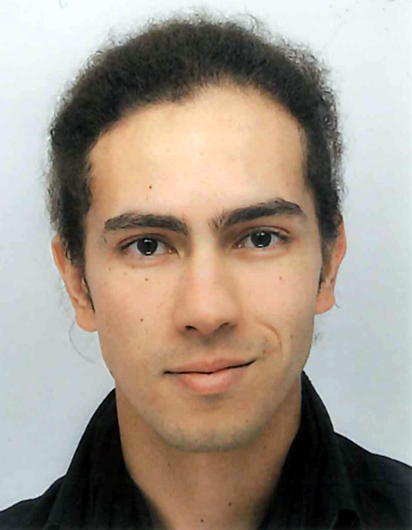
\includegraphics[height=4.cm] {ID_photo.png}
\end{minipage}

%%%%%%%%%%%%%%%%%%%%%%%%%%%%%%%%%%%%%%%%%%%%%%%%%%%%%%%%%%%%%%%%%%%%%%%%%


\vspace{0cm}
{\bf Post-doctorats et situation actuelle :}\\
Mai 2017 - Juin 2020 \rule[-0.4ex]{0.2ex}{1.2em} Bourse FWO $[$Pegasus$]^2$ Marie Sk\l{}odowska-Curie \rule[-0.4ex]{0.2ex}{1.2em} 3 ans \rule[-0.4ex]{0.2ex}{1.2em} KU Leuven\\
Octobre 2016 - Mai 2017 \rule[-0.4ex]{0.2ex}{1.2em} Contrat postdoctoral \rule[-0.4ex]{0.2ex}{1.2em} 8 mois \rule[-0.4ex]{0.2ex}{1.2em} KU Leuven\\

\vspace{-0.2cm}
{\bf Th\`ese :} \textit{Wind accretion onto compact objects}, supervis\'ee par F. Casse \& A. Goldwurm \`{a} l'APC (Paris 7, \'{e}quipe High Energy Astrophysics), soutenue le 7 Septembre 2016 (apr\`es 3 ans). 


%%%%%%%%%%%%%%%%%%%%%%%%%%%%%%%%%%%%%%%%%%%%%%%%%%%%%%%%%%%%%%%%%%%%%%%%%
%%%                RECHERCHE :

\vspace{0.2cm}
{\bf Th\`emes des recherches effectu\'ees : } Compact objects (CO): neutron star (NS), black hole (BH) - Roche lobe overflow (RLOF), wind accretion - High mass (HMXB) and low mass X-ray binaries - Stellar and disc outflows, line-driven winds - Ultra-luminous X-ray sources (ULX)

%\emph{D\'esignez  avec quelques mots clefs repr\'esentatifs votre domaine de recherche} 
%I model mass transfer in binary systems hosting a star and a stellar remnant (compact object or white dwarf), i.e. in X-ray binaries and Cataclysmic variables. It proceeds either via Roche lobe overflow or through the stellar wind. A fraction of the latter can be captured by the compact object in Supergiant X-ray binaries such as Vela X-1. As the flow is accreted, it emits copious amounts of light whose photometric and spectroscopic time-variability suggests structures in the flow I try to identify with numerical simulations of these systems.

\vspace{0.3cm}

%%%%%%%%%%%%%%%%%%%%%%%%%%%%%%%%%%%%%%%%%%%%%%%%%%%%%%%%%%%%%%%%%%%%%%%%%
%%%  METHODOLOGIE :

{\bf M\'ethodologies :}  
Th\'eorie --  Mod\'elisation -- Simulations

\vspace{0.3cm}

{\bf T\^{a}ches de service effectu\'ees et/ou envisag\'ees :}\\
%\emph{ Pr\'ecisez le titre, le service d'observation (ANO1 \`a ANO6), le responsable national et d\'ecrivez succinctement l'activit\'e}
ANO2 SVOM - Bertrand Cordier (CEA) - Avec Jean-Luc Atteia et Olivier Godet (IRAP), caract\'{e}risation de la r\'{e}ponse instrumentale d'ECLAIRs et d\'{e}veloppement d'outils d'analyse de la performance de l'instrument pour le segment sol et l'\textit{ECLAIRs Instrument Center} pour produire les fichiers auxiliaires de calibration n\'{e}cessaires au traitement des donn\'{e}es.\\

\vspace{-0.1cm}

{\bf Enseignements effectu\'es :}\\
\makebox[1.5cm][l]{2018-19} \makebox[7cm][l]{Computational methods for Astrophysics} \makebox[2.5cm][l]{40h cours} \makebox[2cm][l]{5$^{\text{th}}$ year} \makebox[3.5cm][l]{KU Leuven}\\
\makebox[1.5cm][l]{2017-18} \makebox[7cm][l]{Linear Algebra} \makebox[2.5cm][l]{30h TD} \makebox[2cm][l]{1$^{\text{st}}$ year} \makebox[3.5cm][l]{KU Leuven}\\
\makebox[1.5cm][l]{2016-17} \makebox[7cm][l]{Computational methods for Astrophysics} \makebox[2.5cm][l]{60h TD} \makebox[2cm][l]{5$^{\text{th}}$ year} \makebox[3.5cm][l]{KU Leuven}\\
\makebox[1.5cm][l]{2014-16} \makebox[7cm][l]{Classical Mechanics} \makebox[2.5cm][l]{128h TD} \makebox[2cm][l]{1$^{\text{st}}$ year} \makebox[3.5cm][l]{Paris 7}\\ 
\makebox[1.5cm][l]{2013} \makebox[7cm][l]{Physics for Medical studies} \makebox[2.5cm][l]{32h TD} \makebox[2cm][l]{1$^{\text{st}}$ year} \makebox[3.5cm][l]{Paris 7}\\ 
\makebox[1.5cm][l]{2013} \makebox[7cm][l]{Deterministic systems and signals} \makebox[2.5cm][l]{32h TP} \makebox[2cm][l]{4$^{\text{th}}$ year} \makebox[3.5cm][l]{Paris 7}\\ 
%\makebox[1.5cm][l]{2012-13} \makebox[7cm][l]{Private lessons with the company \emph{Cours Thal\`es}}- Paris\\ 
\makebox[1.5cm][l]{2009-10} \makebox[6.9cm][l]{Teaching assistant} \makebox[2.5cm][l]{16h cours} \makebox[4.5cm][l]{high school Gustave Eiffel}\\ 

\vspace{-0.1cm}

{\bf R\'esultats principaux :} \\
\underline{2019:} I proved that discs could be formed around a CO in a HMXB by capture of the wind, without RLOF, with dramatic consequences on the spinning up/down of the accretor. I also proposed a new mechanism for mass transfer in ULX. \underline{2018:} overdense regions form in the wind of hot stars (clumps). I showed that the serendipitous capture of these clumps by an orbiting CO does not account for the time variability of the mass accretion rate we observed in Vela X-1 with Chandra, contrary to previously thought. Additional instabilities in the immediate vicinity of the BH or in the NS magnetosphere are required. \underline{2015-17:} characterization of the structure of the bow shock formed as a CO moves through an ambient medium (mass accretion rate, stability, topology of the inner sonic surface), for instance the wind of a stellar companion.\\

\vspace{-0.1cm}

{\bf Programme de recherche :}  
Mergers between a NS and a BH or another NS can lead to the formation of a an accretion disc around the remnant. \underline{1.} Study of the parameters of this disc and of its evolution as it undergoes accretion onto the remnant at high mass accretion rates (above the Eddington limit). \underline{2.} Analysis of the neutrino-driven and subsequent line-driven outflow from this disc and its interaction with the surrounding ejecta responsible for the kilonova.\\

\vspace{-0.1cm}

{\bf Comp\'etences acquises et points forts de votre candidature :}  
Wide expertise in Computational Astrophysics (e.g. MHD approximate Riemann solvers and flux-limited diffusion for radiative transfer). Improvements of \texttt{MPI-AMRVAC}, a finite volume code to numerically solve the equations of MHD, on an adaptive grid whose geometry can be adapted to the needs of a physical problem. I also gained experience in adjacent domains such as visualization, high performance computing, hardware, cluster and data management, profiling and code optimization.

%\newpage

%%%%%%%%%%%%%%%%%%%%%%%%%%%%%%%%%%%%%%%%%%%%%%%%%%%%%%%%%%%%%%%%%%%%%%%%%

\section*{Publications}
\vspace{0.3cm}

{\bf Nombre de publications de rang A publi\'ees et sous presse:} 11 \\
 
{\bf Nombre de publications de rang A soumises:} 0 \\

{\bf Nombre de communications et/ou de posters pr\'esent\'es \`a des
  conf\'erences:} 14 \\
  
{\bf Autres (participation \`a des ouvrages, rapports techniques, codes, logiciels, sites web, etc...) :}\\ \\
\makebox[1.5cm][l]{2013-18} Developer for the MHD code \texttt{MPI-AMRVAC}\\ 
\makebox[1.5cm][l]{2017} Radio show \emph{Faconde} on scientific outreach (Radio Campus, Bruxelles)\\ 
\makebox[1.5cm][l]{2016} PhD manuscript\\ 
\makebox[1.5cm][l]{2015} Festival of Sciences (Paris 7) and 3D-printing of Roche potentials \\ 
\makebox[1.5cm][l]{2015} Personal webpage\\ 
\makebox[1.5cm][l]{2015} Website of the \emph{Rencontres des Jeunes Physiciens 2015}\\ 
\makebox[1.5cm][l]{2015} Community manager of the \emph{Rencontres des Jeunes Physiciens 2015}\\ 
\makebox[1.5cm][l]{2015} Wolfram demonstration \textit{Trajectory of a Test Mass in a Roche Potential}\\

\vspace{0.3cm}

{\bf Liste des 5 publications de rang A, par ordre d'importance, qui illustrent le mieux votre travail et vos comp\'etences   (avec liens) :}\\ \\
\href{http://adsabs.harvard.edu/abs/2018arXiv181012933E}{[1]} \textbf{El Mellah I.}, Sander A. A. C., Sundqvist J. O. \& Keppens R.\\ 
\emph{	Formation of wind-captured discs in Supergiant X-ray binaries : consequences for Vela X-1 and Cygnus X-1} (2019) - A\&A \\ \\
\href{http://adsabs.harvard.edu/abs/2017arXiv171108709E}{[2]} \textbf{El Mellah I.}, Sundqvist J. O. \& Keppens R.\\ 
\emph{Accretion from a clumpy massive-star wind in Supergiant X-ray binaries} (2017) - MNRAS\\ \\
\href{http://adsabs.harvard.edu/abs/2018arXiv181012937E}{[3]} \textbf{El Mellah I.}, Sundqvist J. O. \& Keppens R.\\ 
\emph{	Wind Roche lobe overflow in high mass X-ray binaries : a possible mass transfer mechanism for Ultraluminous X-ray sources} (2018) - A\&A \\ \\
\href{http://adsabs.harvard.edu/abs/2015MNRAS.454.2657E}{[4]} \textbf{El Mellah I.} \& Casse F. \\ 
\emph{A numerical simulations of axisymmetric hydrodynamical Bondi-Hoyle accretion}\\
\emph{on to a compact object} (2015) - MNRAS\\ \\
\href{http://adsabs.harvard.edu/abs/2017MNRAS.467.2585E}{[5]} \textbf{El Mellah I.} \& Casse F. \\ 
\emph{A numerical investigation of wind accretion in persistent Supergiant X-ray Binaries}\\
\emph{I - Structure of the flow at the orbital scale} (2016) - MNRAS\\ \\

\end{document}
